
\chapter{State of the art}

The present chapter will cover the state of the art of the metabolomics field, focusing on spectral data. This includes the description of the main techniques and their characteristics, discussing some of the computational tools currently available for metabolomics and spectral data analysis. The workflow of data analysis for a metabolomics experiment will be fully covered, including the pre-processing, univariate and multivariate data analysis, feature selection, and data fusion steps.


\section{Techniques}

\subsection{Infrared Spectroscopy}

\acrfull{ir} spectroscopy deals with the \gls{ir} region of the electromagnetic spectrum and is commonly used in the study and identification of chemicals. The \gls{ir} spectrum can be divided in three main regions, namely, the \gls{fir} (400 $ cm^{-1} $ - 100 $ cm^{-1} $), the \gls{mir} (4000 $ cm^{-1} $ - 400 $ cm^{-1} $) and \gls{nir} (13000 $ cm^{-1} $ - 4000 $ cm^{-1} $). The theory is that molecules absorb specific frequencies that are characteristic of their structure, and these frequencies match the transition energy of the bond or group that vibrates. One of the great advantages of this technique lies in the fact that virtually any sample in any state may be studied.

The introduction of Fourier-transform spectrometers have significantly contributed to the advance in \gls{ir} spectroscopy, dramatically improving the quality of \gls{ir} spectra and minimizing the time required to obtain the data. This type of instrument employs an interferometer and exploits the well established mathematical process of Fourier-transformation. \gls{ftir} spectroscopy has distinct advantages over other conventional methods of biochemical analysis in that it is rapid, reliable and requires a relatively small sample size and simple sample preparation procedure \citep{kansiz1999fourier}. 

The output from such instruments is referred to as a spectrum, and it basically consists in a graph of \gls{ir} light transmittance on the vertical axis vs. wavenumber on the horizontal axis (\autoref{spectra}A), usually in $ cm^{-1} $, decreasing from left to right \citep{Stuart2004}.

Many are the applications of \gls{ir} spectroscopy, ranging from the food area to the biological and medical fields, and it has proven to show good results (\autoref{spectroscopies}). Regarding the food industry, this technique has been used in beer quality assessment \citep{polshin2011beer}, in the discrimination of \textit{Alicyclobacillus} strains in apple juice \citep{lin2005rapid}, in honey sample classification according to their adulteration levels \citep{norazian2012hybrid} and in the detection and quantification of milk adulteration \citep{santos2013rapid}.


Regarding the biological and medical fields, \gls{ir} spectroscopy has been widely applied in  chemometrics approaches, including the differentiation of different \textit{Saccharomyces cerevisiae} strains \citep{cozzolino2006combining}, the discrimination of different plant populations \citep{khairudin2014direct, uarrota2014metabolomics}, the discrimination of clinically relevant bacteria \citep{preisner2007fourier} and even fly species identification \citep{de2011barcoding}.


\subsection{Ultraviolet-visible Spectroscopy}

While interaction with \gls{ir} light causes molecules to undergo vibrational transitions, the higher energy radiation in the UV (200 - 400 $ nm $) and visible (400 - 700 $ nm $) range of the electromagnetic spectrum causes many organic molecules to undergo electronic transitions. The concept is that for molecules containing $ \pi $-electrons or non-bonding electrons, photons of \acrfull{uv} light have enough energy to cause their transition between the different electronic energy levels. The wavelength of light absorbed has the energy required to move an electron from a lower energy level to a higher energy level. Because many transitions with different energies can occur, the bands that appear in the spectrum are broadened.

The \gls{uv} spectrum typically has absorbance values on the vertical axis and  wavelength values on the horizontal axis in $ nm $ (\autoref{spectra}B) rather than $ cm^{-1} $ \citep{soderberg2010organic}. Compared with techniques such as \gls{ir}, which produces many narrow bands, \gls{uv} spectroscopy provides a limited amount of qualitative information. Although the spectra produced by this technique do not enable absolute identification of an unknown compound, they are frequently used to confirm the identity of a substance through comparison of the measured spectrum with a reference spectrum \citep{owen1996fundamentals}.

\gls{uv} spectroscopy has been widely used in areas such as the food industry and forensics (\autoref{spectroscopies}). In the food industry, it has been applied in problems regarding for instance the classification of ground roast coffee according to type and conservation state \citep{souto2010uv}, discrimination of tea varieties \citep{kumar2013discrimination}, prediction of wine aging \citep{pereira2011madeira}, wine differentiation and classification \citep{urbano2006ultraviolet} and also in tequila discrimination \citep{barbosa2007uv}.

Regarding forensics, \gls{uv} spectroscopy has been used in the discrimination of blue ball-point pen inks \citep{thanasoulias2003multivariate} and also in soil discrimination \citep{thanasoulias2002application}.

\begin{figure}
	\centering
	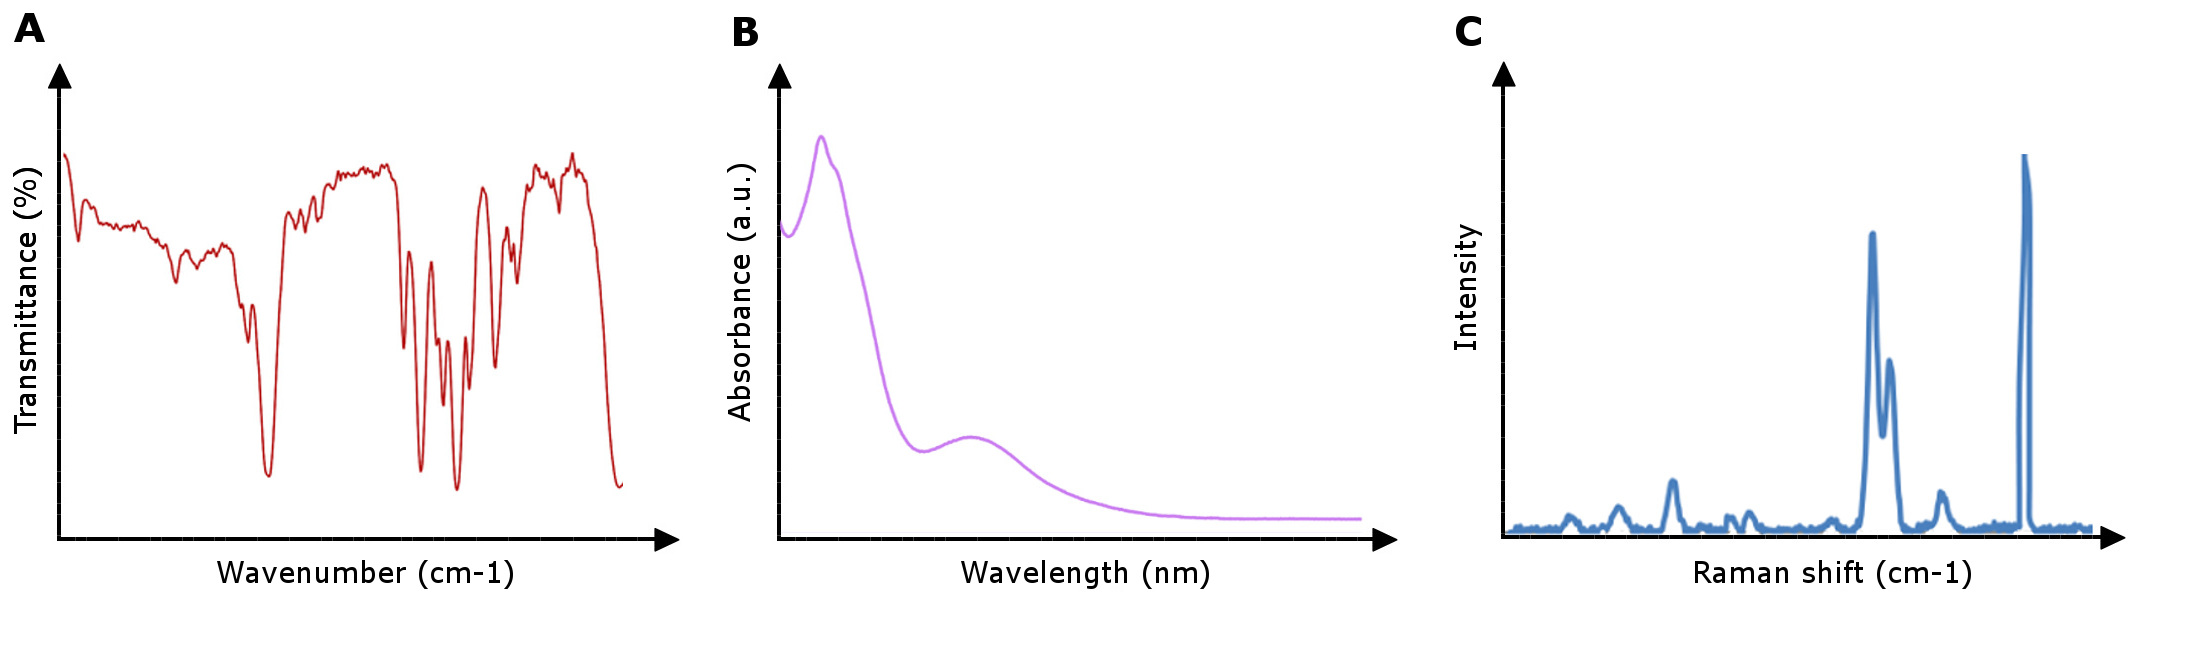
\includegraphics[width=1.1\linewidth]{Imagens/spectroscopies}
	\caption{Example of \acrshort{ir} (\textbf{A}), \acrshort{uv} (\textbf{B}) and Raman (\textbf{C}) spectra with commonly used units represented in the axis.}
	\label{spectra}
\end{figure}

\subsection{Raman Spectroscopy}

Spectroscopies such as Raman are employed to detect vibrational, rotational, and other low-frequency modes in a system. It is widely used to provide information on chemical structures and physical forms, in fingerprinting experiments and even to determine quantitatively or semi-quantitatively a compound in a sample. When light interacts with matter, the photons which make up the light can either be transmitted, reflected, absorbed or scattered, and it is this last tiny portion of light that Raman spectroscopy utilizes.

This technique uses a single frequency of radiation to irradiate the sample, and it is the radiation scattered from the molecule, one vibrational unit of energy different from the incident beam, which is detected. Most of the scattered light does not change its wavelength in the process (Rayleigh scattering) but part of it does, and such scattering is known as Raman scattering. The theory is that Raman scattering of monochromatic light (usually from a laser in the \gls{nir} or \gls{uv} range) is caused by excitations in the system, which result in the energy of the laser photons being shifted up or down. The intensity of the scattered light is plotted against its frequency ($ cm^{-1} $) and the result is a Raman spectrum of the sample (\autoref{spectra}C).

Compared to \gls{ir} spectroscopy, this technique is less widely used, largely due to problems with sample degradation and fluorescence. However, recent advances in instrument technology have simplified the equipment and reduced the problems substantially. These advances, together with the ability of Raman spectroscopy to examine samples in a wide range of states and minimal spectrum manipulation need, have led to a rapid growth in the application of the technique (\autoref{spectroscopies}) \citep{smith2005modern}.

Raman spectroscopy has been widely applied in the forensics area, having proven to be a powerful tool in the identification of body fluids \citep{virkler2010raman, sikirzhytski2010discriminant, sikirzhytski2012advanced}. The pharmaceutical industry also makes use of this technique, addressing problems such as the detection of counterfeit products \citep{roggo2010identification, sacre2011detection} and qualitative and quantitative detection of a mycotoxin in ground maize samples \citep{lee2013application}.




\setcounter{table}{0} %começava em 2 
\newcommand{\htab}[1]{\textbf{{\footnotesize \textcolor{white}{#1}}}}
\definecolor{airforceblue}{rgb}{0.36, 0.54, 0.66}

\begin{scriptsize}
	\begin{longtable}{|m{1.5cm}|m{3cm}|m{1.5cm}|m{4cm}|m{4cm}|}
		%FIRST HEADER------
		\caption{Applications of \acrshort{ir}, \acrshort{uv} and Raman spectroscopies.} 
		\label{spectroscopies} \\
		\rowcolor{airforceblue}
		\htab{Reference} & \htab{Description} & \htab{Techniques} & \htab{Preprocessing} & \htab{Analysis} \\
		\hline
		\endfirsthead
		
		%SECOND HEADER------
		\caption[]{Applications of \gls{ir}, \gls{uv} and Raman spectroscopies. (Continued)} \\
		\rowcolor{airforceblue}
		\htab{Reference} & \htab{Description} & \htab{Techniques} & \htab{Preprocessing} & \htab{Analysis} \\
		\hline
		\endhead
		
		%TABLE--------------
		
		\cite{polshin2011beer} & Prediction of important beer quality parameters & \gls{ftir} & \gls{msc}, Baseline correction, \gls{snv}, 1st
		and 2nd Savitzky-Golay derivatives, Mean centering & \gls{pca}, \gls{plsr} \\ 
		
		\hline 
		\cite{lin2005rapid} & Discrimination of \textit{Alicyclobacillus} strains in apple juice & \gls{ftir} & Spectra smoothing, 2nd derivative, Normalization & \gls{pca}, \gls{simca} \\ 
		
		\hline 
		\cite{norazian2012hybrid} & Classification of honey according to the adulteration level & \gls{ftir} & Baseline correction, Normalization, Peak correction, Outlier removal  & \gls{pca}, \gls{lda},  \\ 
		
		\hline 
		\cite{santos2013rapid} & Detection and quantification of milk adulteration & \gls{mir} & Normalization, 2nd derivative (Savitzky-Golay), Mean centering & \gls{simca}, \gls{plsr} \\ 
		
		\hline 
		\cite{cozzolino2006combining} & Differentiation of different \textit{Saccharomyces cerevisiae} strains & \gls{nir} & Autoscaling, Centering, 2nd derivative & \gls{pca}, \gls{lda} \\ 
		
		\hline 
		\cite{khairudin2014direct} & Discrimination of \textit{Polygonum minus} populations & \gls{ftir} & Pareto scaling & \gls{pca}, \gls{plsda} \\ 
		
		\hline 
		\cite{uarrota2014metabolomics} & Identification of changes and discrimination of cassava samples undergoing \gls{ppd} & \gls{ftir} & Normalization, Baseline correction & \gls{pca}, \gls{plsda}, Hierarchical clustering, \gls{svm}, One-way \gls{anova} \\ 
		
		\hline 
		\cite{preisner2007fourier} & Discrimination between different types of the \textit{Enterococcus faecium} bacterial strain & \gls{ftir} & 1st
		and 2nd Savitzky-Golay derivatives, \gls{msc}, \gls{snv}, Mean centering, Outlier removal & \gls{dipls}, \gls{plca} \\ 
		
		\hline 
		\cite{de2011barcoding} & Identification of fly species in the genus \textit{Neodexiopsis Malloch} & \gls{nir} & Savitzky-Golay derivative and smoothing & \gls{pca}, \gls{pls} \\ 
		
		\hline 
		\cite{kumar2013discrimination} & Discrimination of tea varieties & \gls{nir}, \newline \gls{uv} & Normalization & \gls{pca}, K-means clustering, \gls{pnn}, \gls{ann} \\ 
		
		\hline 
		\cite{souto2010uv} & Classification of coffee extracts according to type and conservation state & \gls{uv} & None & \gls{pca}, \gls{simca}, \gls{spalda} \\ 
						
		\hline 
		\cite{pereira2011madeira} & Prediction of wine aging & \gls{uv} & Mean centering, Smoothing, 1st and 2nd derivatives, \gls{snv}, \gls{osc} & \gls{plsr} \\ 
		
		\hline 
		\cite{urbano2006ultraviolet} & Differentiation and classification of wines & \gls{uv} & 1st derivative & \gls{pca}, \gls{simca} \\ 
		
		\hline 
		\cite{barbosa2007uv} &  Discrimination between classes of tequila & \gls{uv} & 1st derivative, Centering & \gls{pca}, \gls{plsda} \\ 
		
		\hline 
		\cite{thanasoulias2003multivariate} & Forensic discrimination of blue ball-point pen inks & \gls{uv} & Normalization & K-means cluster analysis, \gls{pca}, \gls{da} \\ 
		
		\hline 
		\cite{thanasoulias2002application} & Forensic soil discrimination & \gls{uv} & Normalization & K-means cluster analysis, \gls{pca}, \gls{da} \\ 
		
		\hline 
		\cite{virkler2010raman} & Forensic body fluid identification (blood) & \gls{nir}, \newline Raman & Normalization & \gls{sfa}, \gls{pca}, \gls{als} \\ 
		
		\hline 
		\cite{sikirzhytski2010discriminant} & Forensic identification of blood, semen and saliva stains & Raman & None & \gls{da}, \gls{simca}, \gls{lda}, \gls{plsda} \\ 
		
		\hline 
		\cite{sikirzhytski2012advanced} & Identification of body fluid traces (semen and blood) & \gls{nir}, \newline Raman & Cosmic ray interference removal, Normalization, Baseline correction & \gls{pca}, \gls{sfa}, \gls{svm} \\ 
		
		\hline 
		\cite{roggo2010identification} & Identification of pharmaceutical tablets & Raman & Cosmic ray interference removal, \gls{snv} normalization, Scaling, Mean centering, Savitzky-Golay 1st derivative & \gls{svm} \\ 
		
		\hline 
		\cite{sacre2011detection} & Detection of counterfeit Viagra{\textregistered} & Raman & Normalization & \gls{pca}, \gls{simca}, \gls{knn}, \gls{lda} \\ 
		
		\hline 
		\cite{lee2013application} & Qualitative and quantitative detection of a mycotoxin in ground maize samples & Raman & Background correction, Baseline correction, Normalization, Savitizky-Golay smoothing, Peak deconvolution & \gls{knn}, \gls{lda}, \gls{plsda}, \gls{mlr}, \gls{plsr}, Cluster analysis \\ 
		
		\hline 
		
	
	\end{longtable}
\end{scriptsize}





